%!TEX root = ../main.tex

\chapter{Web新闻采集系统的设计与实现}

\section{概述}
\label{sec:system-intro}

随着互联网资源的爆发式增长,Web新闻的便捷性、广泛覆盖性和自由性给传统媒体带来巨大冲击,
无论是从门户网站上浏览分类新闻,还是从智能手机上接收热点新闻推送,
Web新闻已经成为人们获取信息的重要渠道。

面对每天都飞速增长的Web新闻,如何从中挖掘舆情信息、研究热点事件的产生传播规律,
都有赖于一个渠道来源丰富的Web新闻采集系统的支持。

新闻采集系统的主要目标是,通过多种渠道采集Web新闻,并对原始新闻进行正文及元信息抽取,
转化为结构化信息存储于数据仓库中,并提供全文检索支持,
也为后续的自然语言处理和机器学习提供数据接口。
系统使用了本文提出的基于有效字符的Web内容抽取算法,来进行新闻正文的抽取,
通过系统的运行效果,验证了模板无关的内容抽取算法对爬虫系统的实际意义。

面对海量异构、持续变化的新闻网站,大数据的存储压力,
在设计Web新闻采集系统时,需要考虑以下几个关键问题:

(1)准确性

为了节省存储系统的开销、降低索引规模、也能够为用户提供“干净”的新闻内容,
新闻采集系统并不存储原始HTML网页,而是进行正文及元信息抽取后,存储结构化信息。
这就要求系统的信息抽取算法准确性足够高,保留新闻的核心内容,
而过滤冗余内容和噪声,保证内容的质量。

(2)实时性

新闻内容的重要价值在于实时性,随着时间的流逝其价值会不断降低。
这就要求爬虫系统能够在尽可能短的时间内,将最新发布的Web新闻采集汇总,
提供给用户,保证整个系统的实时性。

(3)可扩展性

面对海量异构、持续变化的新闻网站,可扩展性首先体现在人工成本上。
传统的基于包装器或模板的信息抽取方法难以适应互联网规模的采集要求,
系统应当在扩展采集源时投入尽可能少的人力成本,并且考虑到后续的维护成本,
因此本系统使用了模板无关的信息抽取算法。
其次,面对大数据的存储压力,可扩展性要求系统的存储和检索系统能够随时水平扩展,
通过多机分布的方式抗住压力。

(4)稳定性

稳定性是系统的基本要求,新闻采集系统在后台24小时不间断地从多种渠道采集Web新闻,
并对用户提供检索和其它服务。
在互联网的复杂环境下,系统运行过程中会遇到各种未知情况,
这要求系统能够捕捉异常并正确处理,做好日志记录和监控,保证整个服务的稳定可用性。

本章后续内容安排如下,
~\ref{sec:system-architecture}~节介绍系统的总体设计方案,
对其中的架构方案、工作流程做重点阐述;
~\ref{sec:system-module}~节详细阐述系统主要模块的设计与实现,
包括列表解析模块和信息抽取模块等;
~\ref{sec:system-evaluation}~节对系统的实际运行效果进行评估,
验证信息抽取的效果,测试业务功能;
~\ref{sec:system-conclusion}~节总结本章。

\section{总体设计方案}
\label{sec:system-architecture}

\subsection{系统架构}
Web新闻采集系统的总体架构如图~\ref{fig:architecture}~所示,
标示了系统的关键组件和数据流动情况。

\begin{figure}[htbp]
\centering
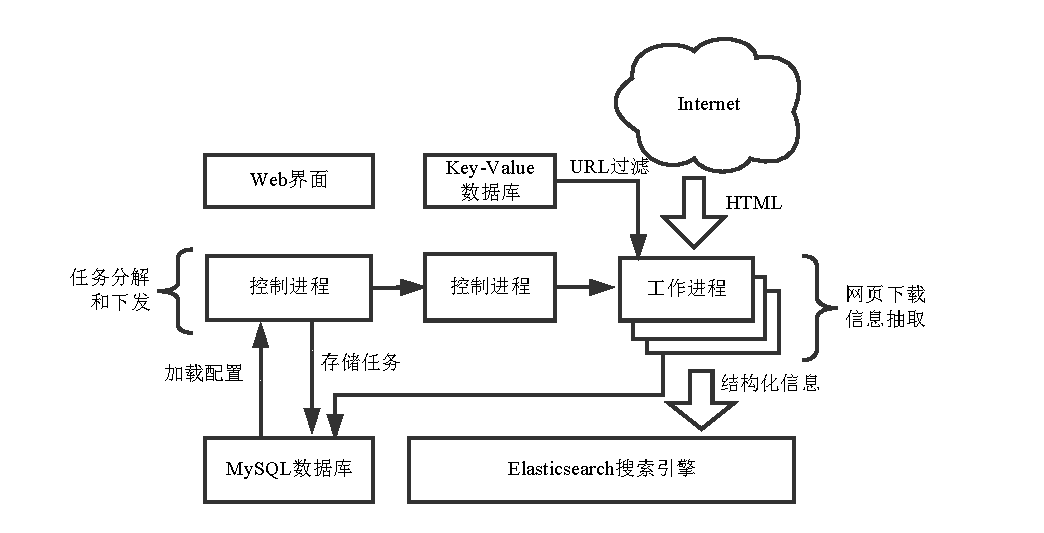
\includegraphics{architecture}
\caption{Web新闻采集系统整体架构}
\label{fig:architecture}
\end{figure}

系统的存储层包括传统关系型数据库MySQL,
Elasticsearch存储与检索引擎,充分发挥了各自的优势。
MySQL负责传统的关系型存储任务,例如配置管理和任务管理,
而ELasticsearch负责结构化信息的存储,能够方便地提供全文检索功能。
Elasticsearch具有很强的扩展能力,多机部署构成集群,面向用户提供透明的HTTP接口,
能够满足存储和检索的分布式扩展需求。

系统的采集层主要包括由Python编写的爬虫模块,分为控制进程和工作进程两类:
控制进程以定时任务或其它方式触发,从MySQL中加载爬虫配置,
将任务分解并下发到消息队列中;
工作进程包括列表解析模块和信息抽取模块,从消息队列中接受任务并执行。
这是一个典型的“生产者-消费者”模型,通过消息队列联系在一起,相互解耦并能灵活地实现并行化。
为了防止重复抓取同一个页面而造成资源浪费,还需要一个全局的URL过滤组件,
判断当前URL是否已经重复,这里使用Key-Value数据库Redis实现。

系统的展示层是一套Web界面,主要包括用户登录界面、采集系统配置界面、
系统运行状态监控界面和新闻检索界面。
在采集系统配置界面,用户可以在多个新闻采集来源中进行选择,并完成具体的配置,
例如RSS地址、新闻URL模式和采集频率等;
通过运行状态监控界面,用户能够直观地了解整个系统的运行情况,
包括采集的新闻总量、各个渠道来源和新闻网站的分布情况、内存硬盘的消耗情况等;
在新闻检索界面中,用户可以提交查询请求,系统借助Elasticsearch的搜索服务,
返回与之相关联的新闻内容。

\subsection{新闻采集流程}
Web新闻从多种信息来源采集,对每一个新闻来源,系统都有与之对应的新闻列表解析模块,
从不同渠道的来源中解析新闻页面URL,转交给信息抽取模块。
这种架构的优势在于,通过消息队列的中转,新闻列表解析和新闻信息抽取相互解耦,
屏蔽底层细节,为信息抽取提供统一的接口,也利于计算资源的水平扩展。

图~\ref{fig:architecture}~表现了控制进程和工作进程的一般关系,
为了详细阐述新闻采集过程,将工作进程细分为新闻列表解析模块,
以及新闻信息抽取模块,形成图~\ref{fig:crawler}~。
其中1--6标示的是各个流程:
\begin{enumerate}
\item 控制进程以定时任务或其它方式触发,从MySQL数据库加载配置,
对每一个新闻来源渠道,数据库都有相应的配置表项;
\item 控制进程分解任务,封装为消息投放到消息队列中,
消息还可以设定相应的优先级和延迟执行时间,从而灵活配置计算资源;
\item 新闻列表解析模块接受任务后从指定的新闻源解析得到一系列新闻URL;
\item 新闻列表解析模块将新闻URL封装成消息投放到消息队列中;
\item 新闻信息抽取模块接受任务后从URL指定的新闻页面中,抽取正文内容及其它元信息;
\item 新闻信息抽取模块将新闻正文内容及其它元信息转储到Elasticsearch搜索引擎中。
\end{enumerate}

\begin{figure}[htbp]
\centering
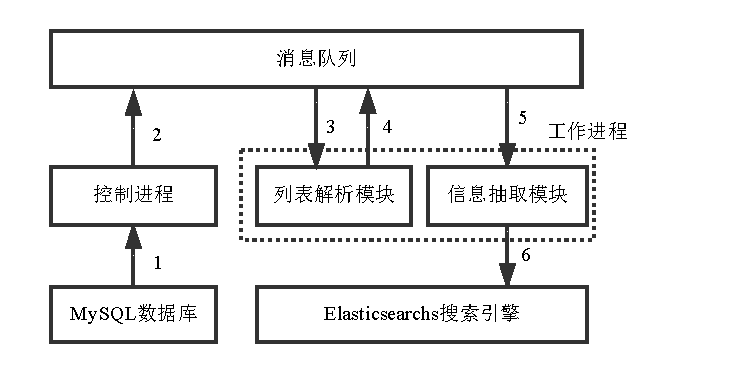
\includegraphics{crawler}
\caption{新闻采集流程}
\label{fig:crawler}
\end{figure}

\section{各模块的设计与实现}
\label{sec:system-module}

\subsection{列表解析模块}
Web新闻采集的来源包括RSS、元搜索和一般新闻网站三类。
RSS是被广泛接受的标准信息聚合接口,这是系统优先考虑的采集来源,
但部分新闻网站可能不提供RSS接口,所以需要针对一般新闻网站的列表解析模块。
元搜索利用现有搜索引擎对新闻的聚合能力,是对热点新闻聚合的一种补充方式。

\subsubsection{RSS}
RSS可以是以下三个解释的其中一个:
\begin{itemize}
\item Really Simple Syndication
\item RDF (Resource Description Framework) Site Summary
\item Rich Site Summary
\end{itemize}

RSS使用一组标准的Web信息流格式来发布频繁更新的信息,如博客、新闻头条和音视频等。
RSS是互联网上被广泛采用的内容包装和投递协议,搭建了一个信息迅速传播的技术平台,
使得每个人都成为潜在的信息提供者。

一个RSS文档包含摘要内容和一些元信息,例如发布日期和作者的名字。
RSS是XML格式的普通文本,简单的格式使得它既能被程序自动化解析也能被普通人理解,
一个RSS如例~\ref{ex:rss}~所示\footnote{https://en.wikipedia.org/wiki/RSS}。

\begin{example}
\label{ex:rss}
RSS示例
\end{example}
\begin{oframed}
\begin{verbatim}
<?xml version="1.0" encoding="UTF-8" ?>
<rss version="2.0">
<channel>
  <title>RSS Title</title>
  <description>This is an example of an RSS feed</description>
  <link>http://www.example.com/main.html</link>
  <lastBuildDate>Mon, 06 Sep 2010 00:01:00 +0000 </lastBuildDate>
  <pubDate>Sun, 06 Sep 2009 16:20:00 +0000</pubDate>
  <ttl>1800</ttl>

  <item>
    <title>Example entry</title>
    <description>Here is an interesting description.</description>
    <link>http://www.example.com/blog/post/1</link>
    <guid isPermaLink="true">7bd204c6-1655-4c27</guid>
    <pubDate>Sun, 06 Sep 2009 16:20:00 +0000</pubDate>
 </item>
</channel>
</rss>
\end{verbatim}
\end{oframed}

在新闻列表解析模块,我们最关心的是新闻页面的URL,即\texttt{<link>}。
通过简单的正则表达式匹配,就能抽取出一组新闻页面的URL,然后提交给新闻信息抽取模块。

\subsubsection{元搜索}
为了利用现有搜索引擎对新闻的聚合能力,系统还采用元搜索的方式获得新闻。
元搜索根据关键词提交查询请求,系统通过维护热点关键词列表,能够及时获得热点新闻,
这对于热点新闻的聚合是一种有效的补充方式。
Web新闻聚合系统面向国内舆情热点,选取了知名的中文搜索引擎百度
\footnote{http://www.baidu.com/}和360\footnote{https://www.so.com/}
作为元搜索入口:
\begin{itemize}
\item http://news.baidu.com/ns?word=\textbf{keyword}\&tn=news\&from=news
\item http://news.so.com/ns?q=\textbf{keyword}\&src=newhome
\end{itemize}

URL中粗体标示的\textbf{keyword}可以替换为搜索关键词,搜索引擎会返回与之相关的新闻。
以百度新闻搜索为例,包含了新闻题目、摘要、发布时间和链接等信息。
通过人工编写的包装器,可以抽取出一组新闻页面的URL,
由于搜索引擎较少,编写包装器的开销并不大。

\subsubsection{一般新闻网站}
RSS基于XML提供了一种统一的信息发布格式,大大降低了聚合信息的代价,
也是系统优先考虑的采集来源。
但仍存在部分新闻网站,不提供RSS接口,我们采用编写包装器的方式解析新闻列表。
因为我们关心的是新闻页面的URL,所以包装器主要包含新闻页面URL的正则表达式。

如表~\ref{tbl:url-pattern}~所示,这是一组新闻页面URL的正则表达式,
其中既包含绝对地址(\verb|http://\w+.cnr.cn/\w+/\w+/\d{8}/\w+.shtml|),
也包含相对地址(\verb|/news/\w+/story\d+-\d+|)。
在新闻列表的HTML页面上匹配相应的URL模式,再根据相对地址、绝对地址进行转换,
就能抽取出一组新闻页面的URL。

\begin{table}[htbp]
\caption{新闻页面URL模式}
\label{tbl:url-pattern}
\vspace{0.5em}\centering\wuhao
\begin{tabular}{lll}
\toprule[1.5pt]
编号 & 新闻网站 & URL模式 \\
\midrule[1pt]
1 & 联合早报 & \verb|/news/\w+/story\d+-\d+| \\
2 & 中国信息网 & \verb|/\w+/\d\d\d\d/\d\d-\d\d/\d+.shtml| \\
3 & 南方网 & \verb|http://\w+.southcn.com/\w+/\d\d\d\d-\d\d/\d\d/content_\d+.htm| \\
4 & 央广网 & \verb|http://\w+.cnr.cn/\w+/\w+/\d{8}/\w+.shtml| \\
5 & 中国军网 & \verb|\d\d\d\d-\d\d/\d\d/content_\d+.htm| \\
\bottomrule[1.5pt]
\end{tabular}
\end{table}

\subsection{信息抽取模块}
新闻信息抽取模块的输入是新闻页面的URL,然后返回抽取的发布日期、标题和新闻正文三元组。
新闻信息抽取流程如图~\ref{fig:news-extract}~所示,在抽取各项信息之前,
还需要检测新闻网页的编码格式,将HTML文档在内存中解析为DOM树。
在信息抽取结束后,还需要判断抽取的三元组是否有效,无效则放弃。

\begin{figure}[t]
\centering
\begin{tikzpicture}[node distance = 2cm, auto]
\node[startstop](init){开始};
\node[io, below of=init](input){新闻URL};
\node[process, below of=input](encoding){编码格式检测};
\node[process, below of=encoding](DOM){DOM树解析};
\node[process, right of=init, xshift=3cm](date){发布日期抽取};
\node[process, below of=date](title){标题抽取};
\node[process, below of=title](content){新闻正文抽取};
\node[decision, below of=content, yshift=-0.5cm](verify){是否有效?};
\node[io, below of=verify, yshift=-0.5cm](output){日期,标题,正文};
\node[startstop, below of=output](stop){结束};

\draw[arrow](init)--(input);
\draw[arrow](input)--(encoding);
\draw[arrow](encoding)--(DOM);
\draw[thick,->] (DOM) -| ++(2,0) |- (date);
\draw[arrow](date)--(title);
\draw[arrow](title)--(content);
\draw[arrow](content)--(verify);
\draw[arrow](verify)--node[near start]{是}(output);
\draw[thick,->](verify) -| node[near start]{否} ++(4,-2) |- (stop); 
\draw[arrow](output)--(stop);
\end{tikzpicture}
\caption{新闻信息抽取流程图}
\label{fig:news-extract}
\end{figure}

\subsubsection{发布日期}
发布日期是构成新闻必不可少的元素,新闻的发布日期一般在标题之下。
通过~\ref{subsec:anchor}~节中提供的日期正则表达式,
可以从HTML文档中抽取日期,从中进行筛选得到最终的发布日期。
发布日期的抽取过程如算法~\ref{algo:extract-date}~所示,
只选择大于某个特定时期(如2016年1月1日),并且在当前时间之前的日期作为候选,
最后从其中选择最近的日期,作为这篇新闻的发布日期。

\begin{algorithm}[htbp]
\caption{extractPubDate(Src)}
\label{algo:extract-date}
\KwIn{HTML Text Src}
\KwOut{Publication date}

candidate\_dates = $\emptyset$ \;
\For{every date string $s$ extracted from Src via regular expression}{
  Build date structure $d$ from date string $s$ \;
  \If{$d$ > 2016/1/1 \textbf{and} $d$ < now()}{
    candidate\_dates.add($d$) \;
  }
}
\eIf{candidate\_dates is not null}{
  \Return maximum(candidate\_dates) \;
}{
  \Return null \; 
}
\end{algorithm}

\subsubsection{新闻标题}
HTML文档中\texttt{<title>}标签表示网页的标题,但它一般不能直接作为新闻的标题。
以~\ref{sec:cevc-intro}~节图~\ref{fig:news}~为例,
这篇新闻的\texttt{<title>}为
\textbf{国务院参事:“建10个类似北京超大城市”是误解|仇保兴|超大城市\_新浪新闻},
但其中包含了分隔符、关键词、新闻网站名称,需要从中过滤这些额外信息。
通过观察发现,新闻的标题一般也会出现在HTML文档的\texttt{<h1>}标签中,
\texttt{<h1>}表示一级标题。
在计算\texttt{<titie>}和\texttt{<h1>}的最长公共子串后,这些额外信息就能被过滤。

为了新闻标题抽取的准确性,我们通过以下步骤确定最终的标题:
\begin{enumerate}
\item 抽取\texttt{<title>}和\texttt{<h1>};
\item 计算\texttt{<titie>}和\texttt{<h1>}的最长公共子串;
\item 如果最长公共子串长度小于5,选取\texttt{<titie>}为标题;
\item 如果\texttt{<titie>}为空,选取\texttt{<h1>}为标题。
\end{enumerate}

\subsubsection{新闻正文}
根据~\ref{sec:cevc-experiment}~节的对比结果,我们选择本文提出的
基于有效字符的Web内容抽取算法CEVC来抽取新闻正文。
CEVC易于实现,预处理阶段依赖小,并且在多个数据集上得到了优于其它对比算法的抽取结果。

\subsection{URL过滤模块}
爬虫在根据系统配置反复抓取的过程中,
需要一个全局的URL过滤模块来判断是否已经处理过当前URL,避免浪费系统资源重复抓取。
针对具体的新闻采集业务,新闻列表URL不能参与过滤,
因为同一个新闻列表页面会不断更新,我们需要反复抓取来获得最新的新闻URL。
需要过滤验重的是具体新闻页面的URL,新闻一经发表不会再改动,它们的URL也是永久链接,
基于此能够达到过滤要求。

系统采用Redis\footnote{http://redis.io/}来实现全局URL过滤模块,
Redis(REmote DIctionary Server)是一个开源的Key-Value存储系统,
使用C语言编写,发行在BSD协议下,与其它Key-Value缓存产品相比具有以下特点:
\begin{enumerate}
\item Redis既可以作为内存型存储,也可以将数据持久化保存在硬盘中,
重启时可以再次加载使用;
\item Redis不仅仅支持简单的Key-Value存储,还提供列表、集合、哈希等高级数据结构;
\item Redis的所有操作都是原子性的,在分布式应用场景下能够保证数据一致性。
\end{enumerate}

最直接的URL过滤方案是使用Redis内置的\texttt{Set}类型,
通过哈希表实现,提供一个string类型的无序集合,集合中不能出现重复数据。
为了提高URL过滤模块存储空间的利用效率,系统采用一种改进的方案:布隆过滤器。

布隆过滤器可以看做是对Bit-Map的扩展,其空间效率很高,
在Redis中由\texttt{GETBIT}和\texttt{SETBIT}实现。
当一个元素被加入集合时,通过K个哈希函数将这个元素映射成一个Bit-Array中的K个位置,
把它们置为1。
在检索时,如果这K个位置都为1,那么该元素\textbf{很可能}存在,
如果这K个位置有任何一个0,那么该元素\textbf{一定不}存在。

布隆过滤器存在误判的现象,具体到新闻采集业务中,就是未被处理过的URL被误判为已经处理过,
但这个概率足够小,一般在万分之一以下,能够被系统接受。
构造布隆过滤器需要提供两个参数,期望容纳的元素个数$n$和误判率$p$,
根据相关公式,能够计算出最优的哈希函数个数。

\subsection{并行调度模块}
在爬虫下载网页的过程中,取决于网络延迟,相当一部分时间花费在等待网站服务器的返回上,
此时工作线程只能阻塞等待。
爬虫采集系统为了保证实时性、提高采集效率,必须充分提高系统的并行度。

采集系统使用“生产者-消费者”的模式,由工作进程统一分解、下发具体的任务,
每个任务都是无状态的,包含执行所需的所有参数。
这样工作进程就能够以幂等的形式存在,只需要关心任务即可,不需要考虑业务之间的状态,
使得工作进程能够通过多机分布式、多进程、多线程的方式简单扩展,不增加额外编程开销。

多个工作进程形成一个“池”,限制了并发规模,在多机部署的时候也能实现负载均衡。
工作进程相互平等,可以接受任意一个网站的抓取任务,
这样不同网站的抓取任务能够随机分布于不同的进程中,防止对单一网站密集抓取而导致的封禁。

爬虫模块由CPython编写,因为CPython存在GIL
\footnote{全局解释器锁,是计算机程序设计语言解释器用于同步线程的工具,
使得任何时刻仅有一个线程在执行},
爬虫模块为了实现真正的并发,使用了多进程的方式,
为了提高进程的利用效率,也可以选择在进程内部运行多线程。

消息队列使用开源的Beanstalkd\footnote{http://kr.github.io/beanstalkd/},
它使用C语言编写,简单而高效。
Beanstalkd支持优先级队列,在采集系统中,我们能够对任务设置不同的优先级,
让实时性更高的任务优先执行,以实现资源的灵活调配。
Beanstalkd还支持延迟消息,这可以利用在爬虫采集过程中,
使得同一个网站的抓取任务保持一定的时间间隔,
防止因为高流量的请求而被网站服务器封禁。

\subsection{存储和检索模块}
由于传统的关系型数据库MySQL对中文全文检索支持不足,且扩展性差,
除了配置管理、任务管理等传统业务存储于MySQL中,
未来增长较快、关系结构简单、需要全文检索的数据则存储于其它数据仓库中。

在对比了Mongodb,Solr和
Elasticsearch\footnote{https://www.elastic.co/}后,
我们选择了Elasticsearch作为数据存储和检索的一体化平台。

Elasticsearch是一个实时的分布式搜索和分析引擎,
它建立在全文搜索引擎框架Apache Lucence
的基础之上,其诞生伊始就完全基于分布式架构。
Elasticsearch可以用于全文搜索、结构化搜索和分析,
在当前互联网上已经有许多成功使用的案例:
\begin{itemize}
\item Github使用Elasticsearch搜索20TB的数据,
包括13亿的文件和1300亿行的代码\citeup{paro2015elasticsearch};
\item Stackoverflow使用Elasticsearch代替SQL全排索引,因为其良好的扩展性和低成本;
\item 维基百科使用Elasticsearch进行全文检索并高亮显示搜索关键词;
\end{itemize}

Elasticsearch为了提供一个扩展性强同时易用的分布式系统,做了许多自动化工作,
例如文档划分到不同容器或者分片中,集群中索引和搜索的跨节点负载均衡,
数据分片的自动冗余备份,无缝衔接的扩展或者恢复整个集群。

Elasticsearch是面向文档的分布式搜索引擎,文档可以代表一个对象。
新闻对象在Elasticsearch中的字段映射如例~\ref{ex:news-mapping}~所示,
其中定义了\texttt{pubdate}为日期类型,\texttt{title}和\texttt{content}为字符串,
\texttt{smartcn}是所使用的中文分词组件。

\begin{example}
\label{ex:news-mapping}
新闻对象的字段映射
\end{example}
\begin{oframed}
\begin{verbatim}
"news": {
  "properties": {
    "url": {"type": "string"},
    "src": {"type": "string"},
    "pubdate": {"type": "date", "format": "yyyy-MM-dd HH:mm:ss"},
    "title": {"type": "string", "analyzer": "smartcn"},
    "content": {"type": "string", "analyzer": "smartcn"}
  }
}
\end{verbatim}
\end{oframed}

\section{运行效果评估}
\label{sec:system-evaluation}

\subsection{测试环境}

Web新闻采集系统的测试环境是一台曙光服务器,
硬件配置如表~\ref{tbl:hard-env}~所示,软件配置如表~\ref{tbl:soft-env}~所示。

\begin{table}[htbp]
\centering
\begin{minipage}{0.45\textwidth}
\caption{系统硬件环境}
\label{tbl:hard-env}
\vspace{0.5em}\centering\wuhao
\begin{tabular}{ll}
\toprule[1.5pt]
硬件 & 型号 \\
\midrule[1pt]
处理器 & AMD Opteron(tm) 6337 HE 6Core 1GHz \\
主板 & Sugon CB60-T Blade 1.0 \\
内存 & 32G \\
硬盘 & 320G \\
网卡 & Intel 82576 Gigabit Network Connection \\
\bottomrule[1.5pt]
\end{tabular}
\end{minipage}
\hfill
\begin{minipage}{0.45\textwidth}
\caption{系统软件环境}
\label{tbl:soft-env}
\vspace{0.5em}\centering\wuhao
\begin{tabular}{ll}
\toprule[1.5pt]
软件 & 版本 \\
\midrule[1pt]
Linux CentOS & 7.0 \\
Python & 2.7.10 \\
MySQL & 5.6.27 \\
Elasticsearch & 2.3.3 \\
Redis & 3.2.0 \\
Beanstalkd & 1.10 \\
Apache & 2.4.20 \\
\bottomrule[1.5pt]
\end{tabular}
\end{minipage}
\end{table}

\subsection{新闻采集统计}

系统从2016年6月8日至17日,平均每天采集2000条新闻,
涉及政治、经济和时事等各个方面。
新闻数量TOP 10的网站分布如图~\ref{fig:site-breakdown}~所示,
新闻采集量最多的网站依次是中国新闻网、环球网、南方网、新华网和凤凰资讯。

\begin{figure}[htbp]
\centering
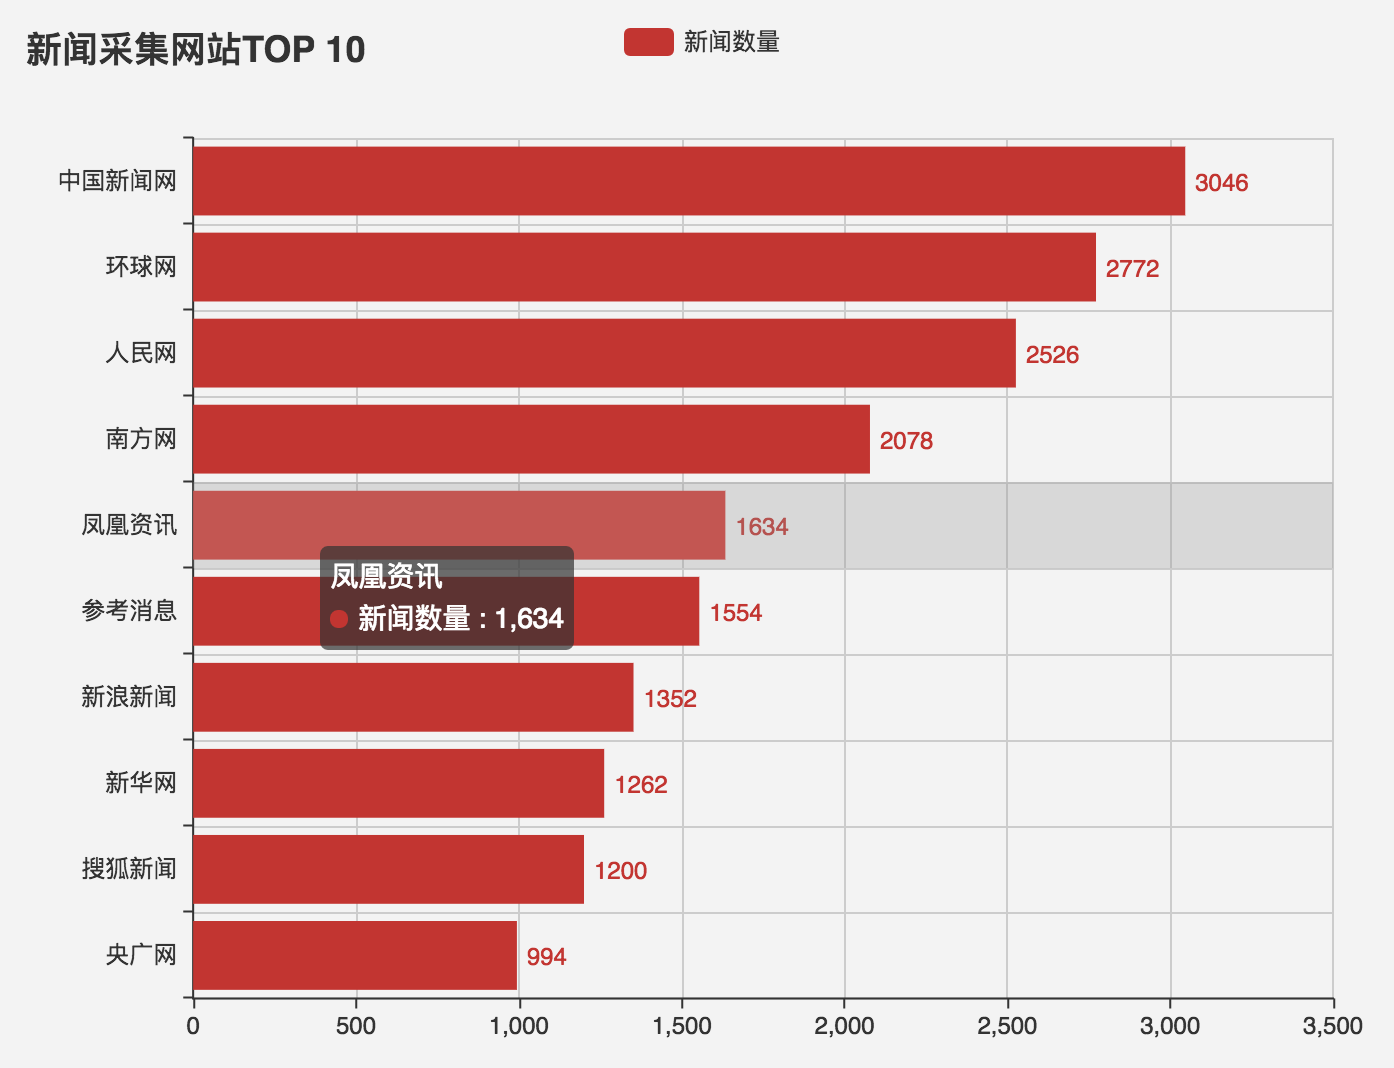
\includegraphics[width=0.9\textwidth]{site-breakdown}
\caption{新闻采集网站TOP 10}
\label{fig:site-breakdown}
\end{figure}

\subsection{新闻信息抽取测试}

为了评估新闻信息抽取模块的准确率,我们从系统采集的新闻中随机抽取200篇,
根据系统中保存的URL访问原始新闻网页,验证各项信息是否抽取正确。
标题和发布日期很容易判断是否正确,记录正确抽取的数量即可。
对于新闻正文的抽取效果,分为两项指标来判断:
\begin{enumerate}
\item 抽取内容是否包含新闻正文;
\item 抽取内容是否基本上只包含新闻正文,即噪声部分比例很小。
\end{enumerate}
这两项指标易于人工审核,也兼顾了精确率和召回率。

最终结果如表~\ref{tbl:sys-evaluation}~所示。
新闻标题通过\texttt{<title>}和\texttt{<h1>}联合确定,
在新闻网页中基本都符合这个规律,所以在样本中准确率达到了100\%。
而发布日期的判断不够严谨,可能被网页中的其它日期干扰,影响了最终的准确率。

需要注意的是,新闻信息抽取模块在抽取标题、发布日期和新闻内容三元组后,
进行了简单的有效性判断(标题多于5个字,发布日期有效,新闻内容多于100个字)。
这使得系统在采集过程中,丢弃了部分新闻,可能是由于正当的原因(URL失效,非新闻网页),
也可能由于信息抽取的失败,所以表~\ref{tbl:sys-evaluation}~中的结果要优于实际情况。

包含正文的准确率为96\%,基本只包含正文的准确率为91\%,
这个结果相对于~\ref{sec:cevc-experiment}~节表~\ref{tbl:cevc-cevc}~中的指标,
99.1\%的召回率和95.8\%的精确率,都有一定差距。
这是因为这里的测试是针对单篇新闻的,没有按字符计算,要求更加严格。
一篇新闻如果没有正确抽取出全部正文,就不能认为包含正文,
而在按字符统计的过程中,依然把正确抽取的内容计算到召回率中。
另外,测试样本较少也是一个因素。

\begin{table}[htbp]
\caption{新闻信息抽取效果评估}
\label{tbl:sys-evaluation}
\vspace{0.5em}\centering\wuhao
\begin{tabular}{llll}
\toprule[1.5pt]
抽取项目 & 总数量 & 正确数量 & 准确率 \\
\midrule[1pt]
标题 & 200 & 200 & 100\% \\
发布日期 & 200 & 191 & 95.5\% \\  
包含正文 & 200 & 186 & 93\% \\
基本只包含正文 & 200 & 182 & 91\% \\
\bottomrule[1.5pt]
\end{tabular}
\end{table}

\subsection{新闻检索测试}

\begin{figure}[htbp]
\centering
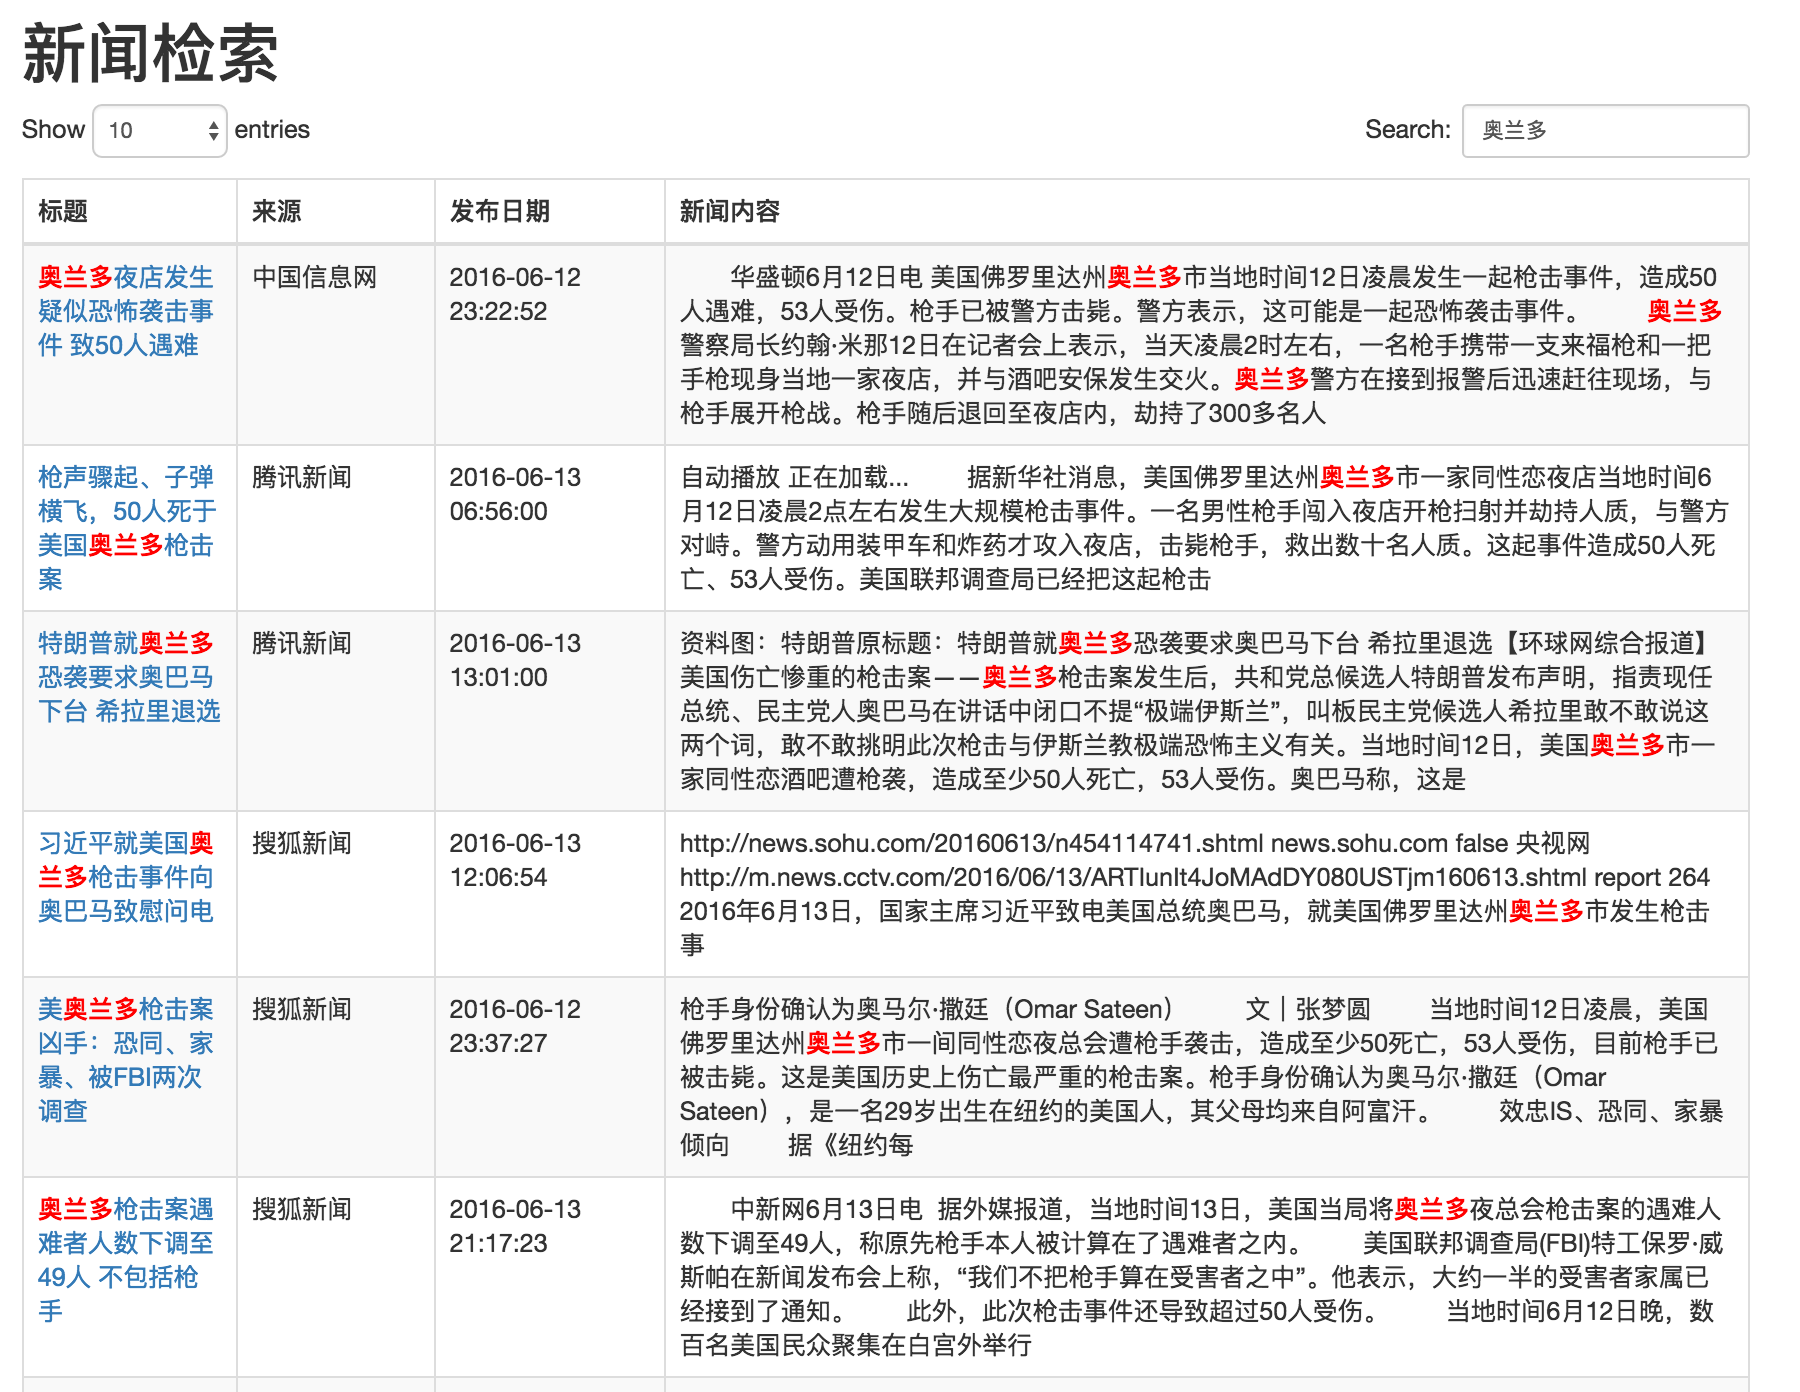
\includegraphics[width=0.9\textwidth]{web-ui}
\caption{新闻检索界面}
\label{fig:web-ui}
\end{figure}

新闻检索界面如图~\ref{fig:web-ui}~所示,
在检索框输入关键词“奥兰多”,系统返回与之关联的新闻,并对关键词进行高亮处理。
表格中只给出了新闻内容的部分片段,点击新闻标题,
能够进入一个独立的页面,详细展示全部新闻内容。
借助于Elasticsearch,系统能够从数据仓库中匹配标题或正文包含搜索关键词的新闻,
并按照相关性的高低排序返回结果。
Elasticsearch使用了高效的索引结构,系统对关键词查询的响应时间在0.5秒以内,
能够适应实时检索的要求。

\section{本章小结}
\label{sec:system-conclusion}

Web新闻采集系统使用了模板无关的内容抽取算法CEVC,
并结合一些领域规则抽取标题、发布日期,
不需要对新闻页面单独构造包装器,大大降低了系统扩展和维护的成本。

系统从RSS、元搜索和一般新闻网站三个信息来源采集新闻,
通过模板无关的抽取技术整合了各个渠道的差异,使人工成本限制在新闻列表解析中。
借助于RSS的统一协议和元搜索技术,新闻列表解析中人工配置和包装器构造的成本能够接受。
系统的后续工作将集中于如何自动扩展新闻采集来源,进一步降低人工参与的成本,
实现系统的高度自动化。
